%!TEX program = xelatex

\documentclass[12pt,a4paper]{article}
\usepackage{xeCJK}
\usepackage{amsmath}
\setCJKmainfont{STSongti-SC-Regular}
\usepackage{setspace}
\usepackage{caption}
\usepackage{graphicx, subfig}
\usepackage{float}
\begin{document} 

\title{homework1}
	\author{11611118 郭思源}  

	\noindent {\Large \textbf {Question 1}} :\\

	\large {我是一个生物信息学专业的学生,主要的研究方向是对单细胞转录组的测序数据进行挖掘,对复杂组织的内部细胞结构和分布进行分析,并研究该组织内的细胞发育过程和各个细胞发育状态对应的标志物。\\


	在进行科研工作的过程中,我发现我的工作本质上就是对特定的组织的生物学组成以及发育方式进行建模,并对转录组测序产生的大量数据进行数据挖掘。而在我最近的一个课题中,我的工作本质上就是对一组高维数据进行合理的降维,并通过数值分析手段取得拟合曲线并通过这个曲线和各个离散的点分析癌细胞的发育路径。通过这个课题,我意识到我需要补充一些数学建模的知识和相关的基本技能,所以我选择了这门课程。\\}
	
	\newpage
	\noindent {\Large \textbf {Question 2}} : \\

	\noindent \large {我阅读的文献为:\\\\
	\textit
	{Global dynamics of a mathematical model for HTLV-I infection of CD4$^+$ T$-$cells}  \\\\
	介绍:\\
	

	人类T细胞嗜淋巴细胞病毒I(HTLV-I)是一种单链RNA逆转录病毒,与成人T细胞白血病(ATL)的发生有关。HTLV-I感染是通过细胞间接触实现的。为了描述HTLV-I感染T细胞的动力学过程和ATL的疾病发展路径,Stilianakis和Seydel首先提出了一个数学模型。该模型由一个非线性常微分方程系统组成,将CD4+T细胞分为四个部分:未感染的CD4$^+$T细胞、潜伏性感染细胞、发病性感染细胞和白血病细胞。\\
	其中T、T$_L$、T$_A$和T$_M$分别表示相应隔室中的细胞数量。\\
	模型的公式如下:\\}
		
	\begin{equation}
	\begin{aligned}
	T' &= \Lambda - \mu_{T}T - \kappa T_{A}T\\\\
	T'_{L} &= \kappa T_{A}T - (\mu_{L} + \alpha)T_{L}\\\\
	T'_{A} &= \alpha T_{L} - (\mu_{A} + \rho)T_{A}\\\\
	T'_{M} &= \rho T_{A} - \beta T_{M} \Bigl( 1 - \frac{T_{M}}{T_{M_{\max}}} \Bigr) - \kappa T_{A}T\\\\
	R_{0} &= \frac{\alpha \kappa T_{A} \Lambda}{\mu_{T} (\mu_{L} + \alpha) (\mu_{A} + \rho) }\\\\
	\end{aligned}
	\end{equation}

	\large
	{其中$\Lambda$是来自前体的CD4$^+$T细胞来源,参数$\mu_{T}$,$\mu_{L}$,$\mu_{A}$
	和$\mu_{M}$分别代表未感染,潜伏感染,活跃感染的CD4$^+$T细胞和ATL细胞的死亡率或去除率。
	参数$\alpha$是潜伏感染的CD4$^+$T细胞变得活跃感染的传播速率,$\kappa$是感染率,
	$\rho$是活跃感染的CD4$^+$T细胞转化为ATL细胞的传播速率。所以,1/$\alpha$和1/$\beta$ 可分别被视为平均潜伏期和感染期. ATL细胞的生长服从速率为$\beta$的经典对数生长函数,$T_{M_{\max}}$是ATL细胞增殖的最大数量。假设模型中的所有参数都是正的常数。\\

	\noindent 模型改进:\\
	

	许多作者采用双线性发病率和标准发病率(也称为比例混合发生率)。然而,上述发病率可能需要改变的原因有多种。其中的一种感染饱和响应引起的非线性发生率已被纳入上述模型中。该模型以下列形式呈现:\\


	\begin{equation}
	\begin{aligned}
	T' &= \Lambda-\mu_{T}T-\kappa \Bigl( \frac{T_{A}}{1+\alpha_{1}T_{A}} \Bigr) T\\\\
	T'_{L} &= \kappa\Bigl(\frac{T_{A}}{1+\alpha_{1}T_{A}} \Bigr)T-(\mu_{L}+\alpha) T_{L}\\\\
	T'_{A} &= \alpha T_{L} - (\mu_{A} + \rho)T_{A}\\\\
	T'_{M} &= \rho T_{A}-\beta T_{M} \Bigl( 1 - \frac{T_{M}}{T_{M_{\max}}} \Bigr)- \mu T_{M}\\\\
	R_{0} &= \frac{\alpha \kappa \Bigl( \frac{T_{A}}{1 + \alpha_{1} T_{A}} \Bigr) \Lambda}{\mu_{T} (\mu_{L} + \alpha) (\mu_{A} + \rho)}\\\\
	\end{aligned}
	\end{equation}




	通过研究上述模型的动力学行为,
	他们观察到基本再生数$R_{0}$可以确定T细胞感染的全局动态,
	即,如果$R_{0}\leq1$,感染的T细胞总是消失。
	如果$R_{0}>1$,则独特的感染平衡在可行区域内部是全局稳定的。在我们的模型中,
	假设发病率为$\kappa f(T_{A}) T$形式,其中$\kappa$是感染率,
	其解释了HTLV-I繁殖的总体效应,例如接触率和感染性。因此,此模型又可以修改为以下形式:\\

	\begin{equation}
	\begin{aligned}
	T'_{ } &= \Lambda-\mu_{T}T-\kappa f(T_{A}) T\\\\
	T'_{L} &= \kappa f(T_{A}) T - (\mu_{L} + \alpha)T_{L}\\\\
	T'_{A} &= \alpha T_{L} - (\mu_{A} + \rho)T_{A}\\\\
	T'_{M} &= \rho T_{A} - \beta T_{M} \Biggl( 1 - \frac{T_{M}}{T_{M_{\max}}} \Biggr)-\mu T_{M}\\\\
	R_{0} &= \frac{\alpha \kappa f'(0) \Lambda}{\mu_{T} (\mu_{L} + \alpha) (\mu_{A} + \rho) }\\\\
	\end{aligned}
	\end{equation}


	\noindent \\\\在这个模型中,函数$f(T_{A})$满足如下性质:\\\\
	$f(0)$ = 0, $f'(T_{A}) > 0$, $f''(T_{A}) \leq 0$\\

	显然,最终的模型中的的发生率包含双线性和饱和发生率。因此,模型3是模型1和2的扩展。在本文中,作者对模型3进行了全局分析。我们将特别的通过构造一个合适的Lyapunov函数而不是利用几何方法来显示模型3的均衡的全局稳定性。\\

	\noindent 下面是对模型3系统的可视化分析:\\
	(1)假设$R_0\leq1$:\\
	\begin{figure}[H]
		\centering
		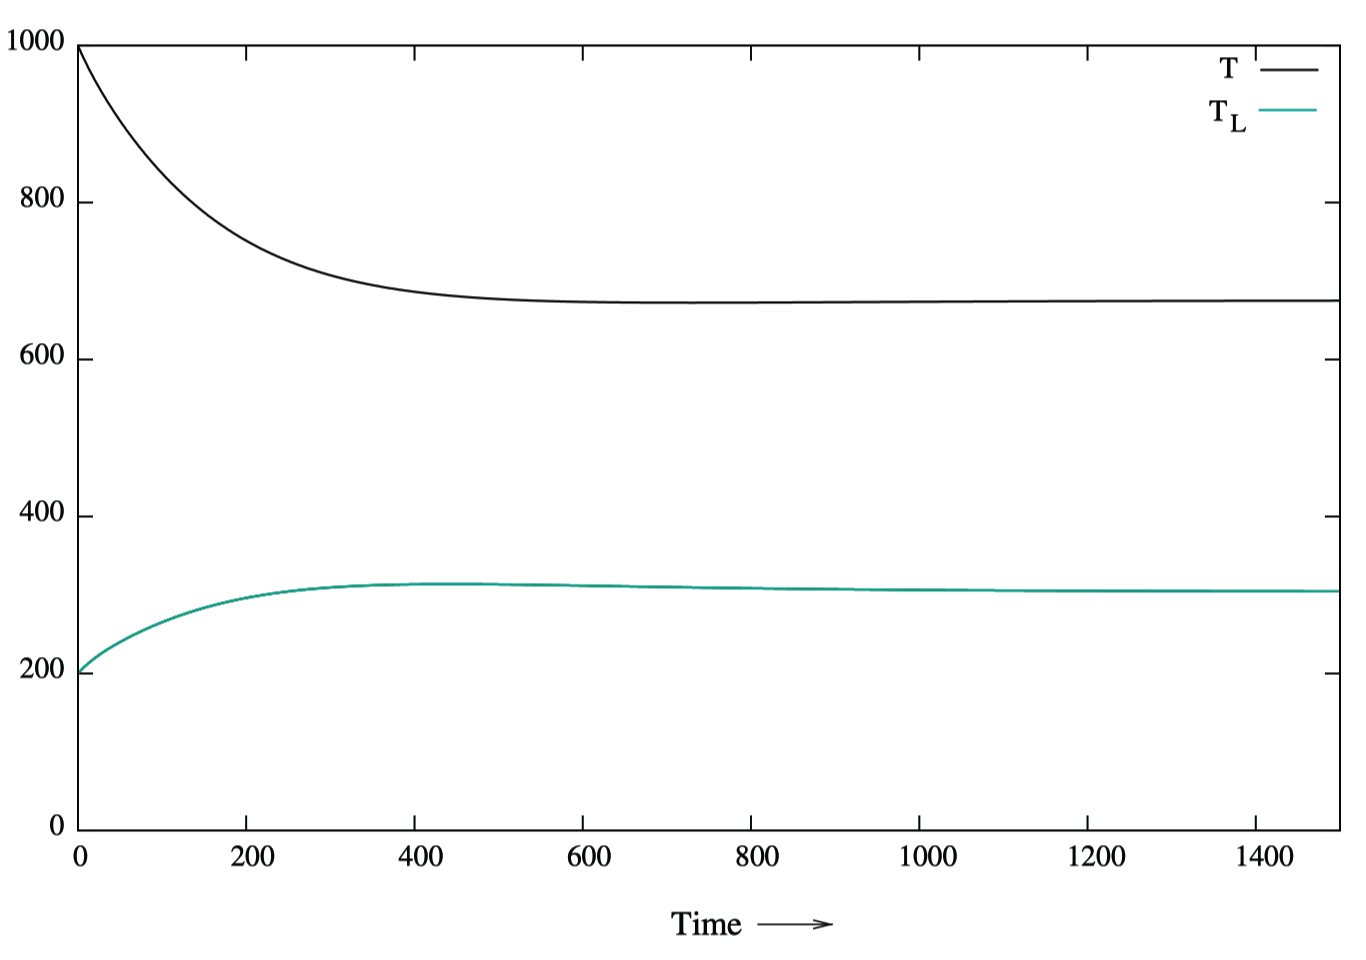
\includegraphics[width=4.5in]{Snip20190310_4.png}
		\caption
		{$T,T_{L}$随时间的变化显示参数值的慢性感染平衡的稳定性,参数为:
		$\Lambda=6,\mu_{T}=0.0006,k=0.1, a=0.1,b=6,\mu_{L}=0.006,\alpha=0.0004,
		\mu_{A}=0.05,\rho=0.00004,\beta=0.0003,\mu_{M}=0.0005,T_{M_{max}}=2200$}
	\end{figure}

	\begin{figure}[H]
		\centering
		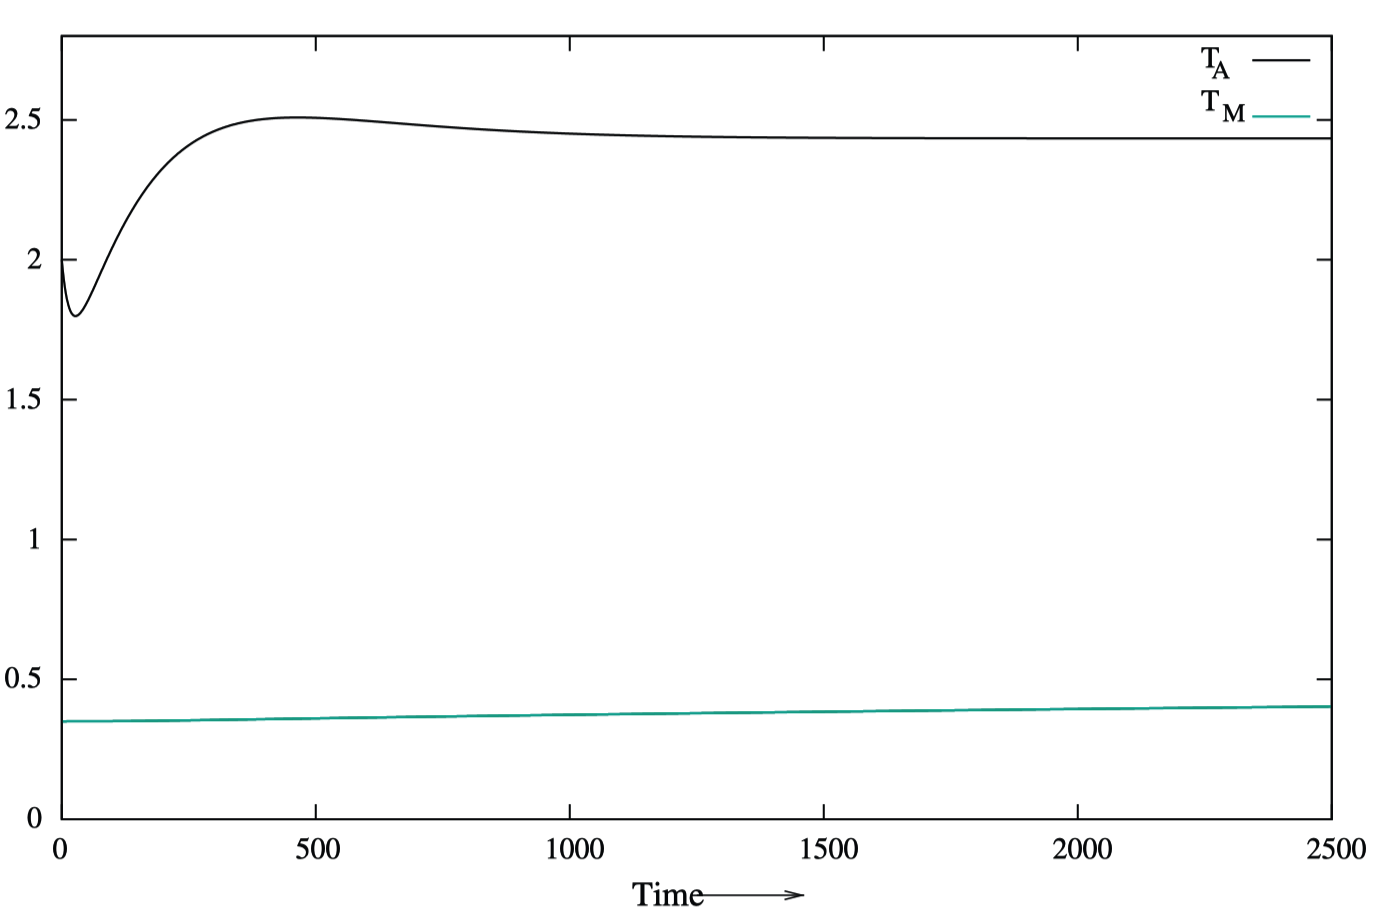
\includegraphics[width=4.5in]{Snip20190310_5.png}
		\caption
		{$T_{A},T_{M}$随时间的变化显示参数值的慢性感染平衡的稳定性,参数为:
		$\Lambda=6,\mu_{T}=0.006,k=0.1, a=0.1,b=6,\mu_{L}=0.006,\alpha=0.0004,
		\mu_{A}=0.05,\rho=0.00004,\beta=0.0003,\mu_{M}=0.0005,T_{M_{max}}=2200$}
	\end{figure}

	\begin{figure}[H]
		\centering
		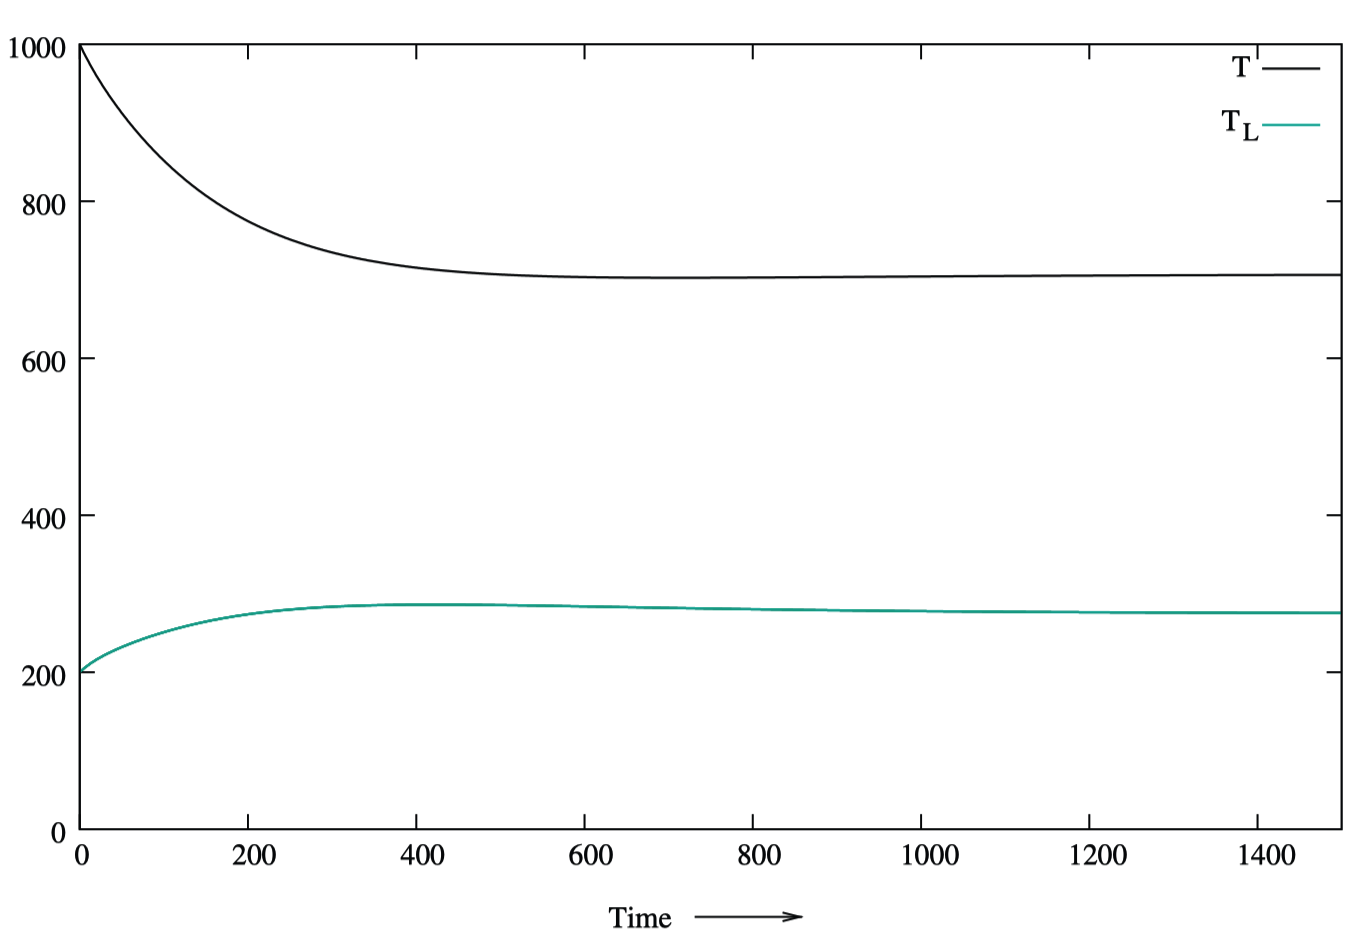
\includegraphics[width=4.5in]{Snip20190310_6.png}
		\caption
		{$T,T_{L}$随时间的变化显示参数值的慢性感染平衡的稳定性,参数为:
		$\Lambda=6,\mu_{T}=0.006,k=0.1, a=0.07,b=0.2,\mu_{L}=0.006,\alpha=0.0004,
		\mu_{A}=0.05,\rho=0.00004,\beta=0.0003,\mu_{M}=0.0005,T_{M_{max}}=2200$}
	\end{figure}
	
	\begin{figure}[H]
		\centering
		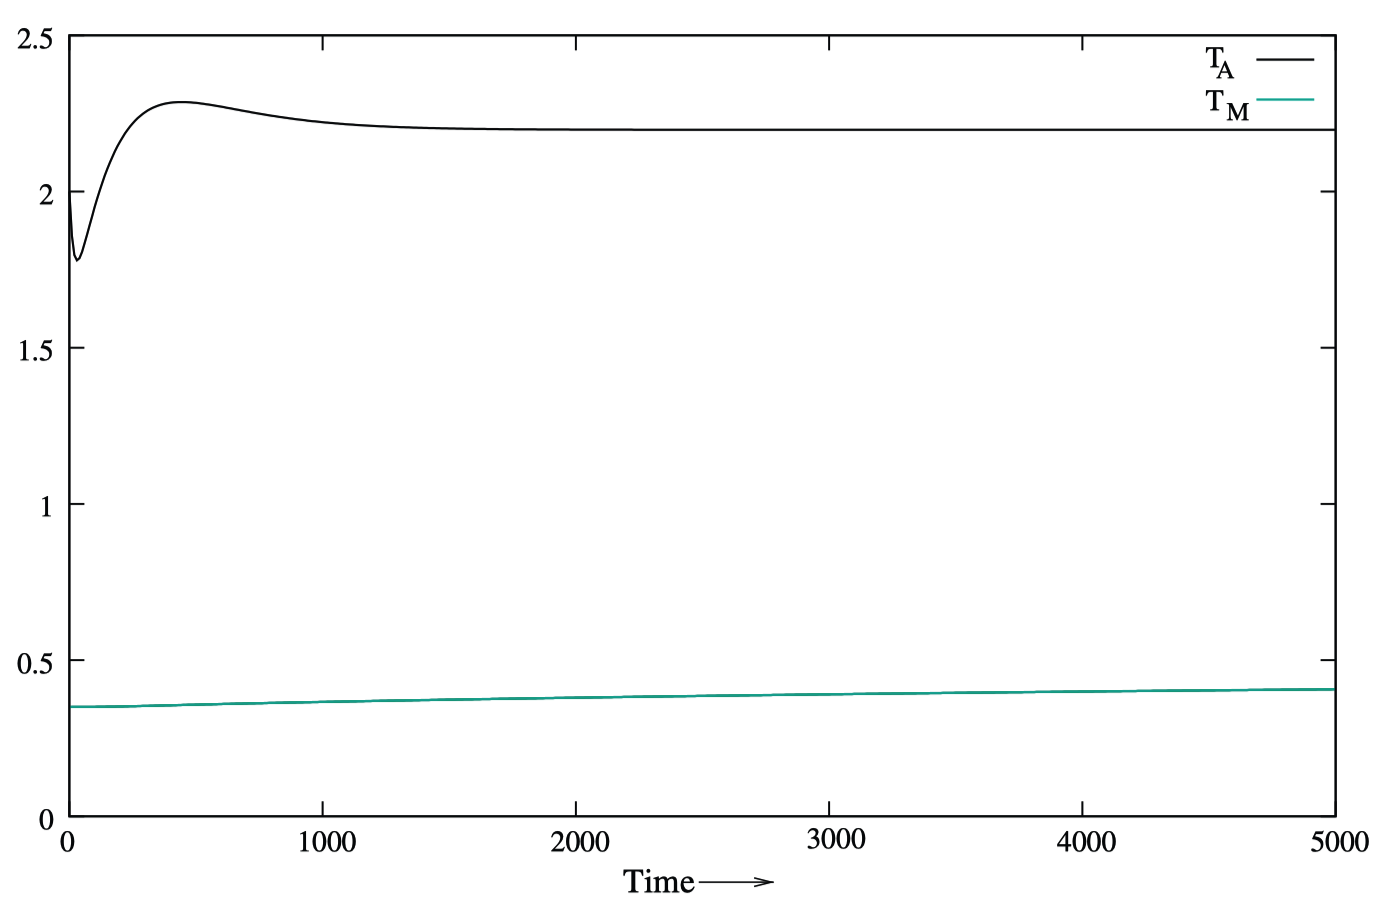
\includegraphics[width=4.5in]{Snip20190310_7.png}
		\caption
		{$T,T_{L}$随时间的变化显示参数值的慢性感染平衡的稳定性,参数为:
		$\Lambda=6,\mu_{T}=0.006,k=0.1, a=0.07,b=0.2,\mu_{L}=0.006,\alpha=0.0004,
		\mu_{A}=0.05,\rho=0.00004,\beta=0.0003,\mu_{M}=0.0005,T_{M_{max}}=2200$}
	\end{figure}

	\begin{figure}[H]
		\centering
		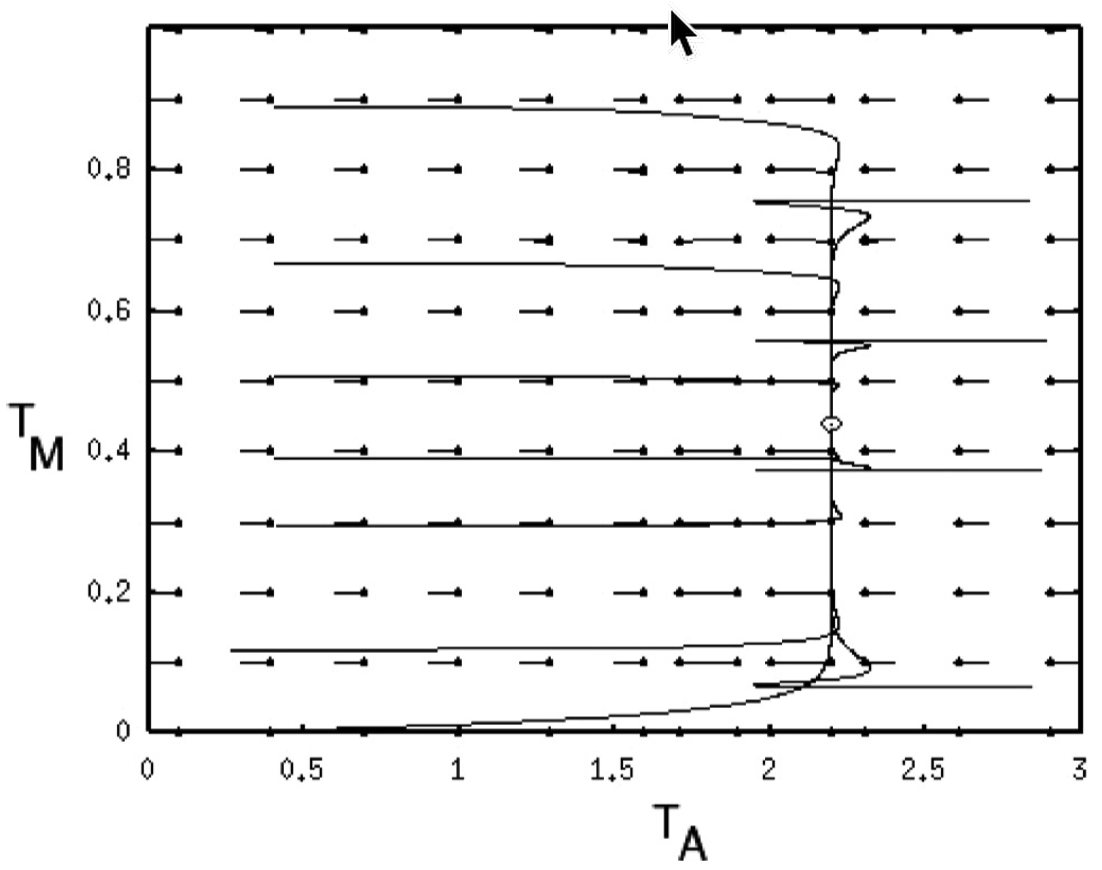
\includegraphics[width=4.5in]{Snip20190310_8.png}
		\caption
		{$T_{M}对T_{A}$的相图显示慢性感染平衡的稳定性,参数为:
		$\Lambda=6,\mu_{T}=0.006,k=0.1, a=0.07,b=0.2,\mu_{L}=0.006,\alpha=0.0004,
		\mu_{A}=0.05,\rho=0.00004,\beta=0.0003,\mu_{M}=0.0005,T_{M_{max}}=2200$}
	\end{figure}

	\noindent 结论:


	在对人类T细胞嗜淋巴细胞病毒I感染的过程所建立的三个模型中,系统的的全局动力学特性完全由基本繁殖数$R_{0}$确定。\\\\

	\newpage
	\noindent{\Large \textbf {Question 3}} : \\

	\large{
	在之前的学习中,我的主要学习内容还是集中在计算机知识和生物学知识上。虽然选修了概率论与数理统计以及常微分方程,但是由于本质上我们还是一个研究生物问题的专业,缺乏应用学会的数学知识的实际背景,导致本来就掌握得不牢靠的数学基础知识没有得到巩固和练习。在进行一些数据分析的时候,我和我的同学们更多的还是将一些统计学方法当作一个黑箱来使用,并没有注重于理解这些统计学工具背后的数学机理,也没有去手工推导过一些很重要的数学结论和定理。\\

	我希望这个学期选修的数学建模课可以作为一个契机,让我有机会回忆起以前学过的数学知识并且重新整合他们,并且我也愿意去掌握更多的新的数学知识和技术来提升自己的能力。同时,我也希望也可以加强自己的编程能力和对数学建模这件事也能有更深入的了解,并拥有完整的数学建模项目的经历。我相信这种基于项目的学习带给我们的压力和成长是同样巨大的。\\

	同时我也发现\LaTeX 和Markdown都是非常有用的提升论文书写效率和提升团队交流效率的工具,虽然这两款工具的初期学习曲线都会一定的坡度,我依然认为这是两个非常有必要掌握的工具。我也愿意在生物信息学的同学们中间宣传这两款工具。\\

	在以前的学习中,我也没有太过于注重实用Matlab这个工具,因为其自带的生物信息学工具包具有局限性。但是我现在发现Matlab十分便于个性化的建模和计算,我会在以后的学习过程中不断熟练自己的Matlab技术。我相信这可以字以后的看就过程中提高我的效率并帮我解决很多的难题。

	}



\end{document}


